\chapter{Bewerten von Anwendungsregeln}
\label{chap:kapitel2}

Anwendungsregeln sind Anforderungen, die der Kunde oder das Projekt, das die jeweilige Komponente oder das Teilsystem einsetzt, zu beachten hat. 
Diese Regeln müssen erfüllt werden, um einen sicheren und zuverlässigen Einsatz jeder Komponente im System zu gewährleisten \cite[S.9]{q2}. 
Dabei können Anwendungsregeln auch sicherheitsrelevant sein. Ist dies der Fall, werden sie auch sicherheitsrelevante Anwendungsregeln genannt. Eine Anforderung wird nach der 
IEEE entweder definiert als eine Bedingung oder eine Fähigkeit, die ein Benutzer benötigt, um ein Problem zu lösen oder ein Ziel zu erreichen oder als eine Bedingung oder Fähigkeit, 
die ein System oder eine Systemkomponente erfüllen oder besitzen muss, um einen Vertrag, eine Norm, eine Spezifikation oder ein anderes formal vorgeschriebenes Dokument 
zu erfüllen \cite[S.62]{q4}. Somit stellen Anwendungsregeln eine besondere Form von Anforderungen dar. Eine sicherheitsrelevante Anwendungsregel 
für ein Zugbeeinflussungssystem könnte wie folgt aussehen:

\begin{quotation}
	\textit{Beispiel Anwendungsregel} \glqq In order to prevent accidents normally covered by Train Control System, the driver shall assume full safety responsibility for the operation of a train if he / she activates a cab on a vehicle 
    with cut-off switch in \glqq ATP off\grqq{} position. If the cut-off switch on a cab is in \glqq ATP off\grqq{} position, the Rolling Stock cut-off-circuitry bypasses all safety related outputs of the 
    Train Control System.\grqq{} \cite[S.7]{q1}.
\end{quotation}

Nutzt ein Projekt nun ein anderes System oder eine andere Komponente, muss der Requirements Manager, also derjenige im Projekt, der sich um das Anforderungsmanagement kümmert, 
die Anwendungsregeln des Systems oder der Komponente im Anforderungsmanagement-Tool IBM Doors importieren und diese bewerten. Die Anwendungsregeln von bereits vorhandenen Systemen 
und Komponenten liegen zentral gespeichert bei IBM Doors. Bei dieser Bewertung muss der Requirements Manager prüfen, ob die importierten Anwendungsregeln im Projekt berücksichtigt 
werden müssen oder nicht. Ebenfalls muss der Requirements Manager ein Statement abgeben, wie er zu dieser Bewertung gekommen ist. Eine Anwendungsregel und ihre Bewertung können der 
Abbildung \ref*{fig:Bewertete Anwendungsregel} entnommen werden.

\begin{figure}[h]
    \centering
    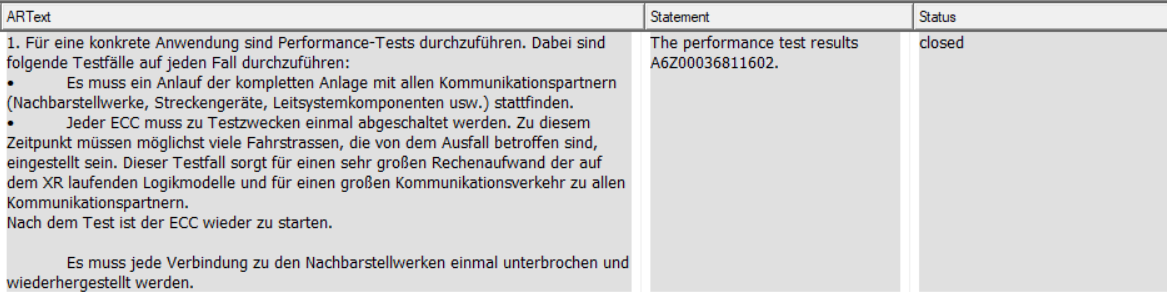
\includegraphics[width = \textwidth]{abbildungen/Bewertete Anwendungsregel.PNG}
    \caption{Beispiel einer bewerteten Anwendungsregel in Doors}
    \label{fig:Bewertete Anwendungsregel}
\end{figure}